\documentclass[12pt,a4paper,titlepage]{article}
\usepackage{fullpage}
\usepackage{hyperref}
\usepackage[pdftex]{graphicx}
\bibliographystyle{plain}
\newcommand{\HRule}{\rule{\linewidth}{0.5mm}}
\usepackage{url}
\usepackage{amsmath}
\usepackage{enumitem}
\usepackage{float}
\usepackage{graphicx}
\usepackage{caption}
\usepackage{subcaption}
\usepackage{tabularx}
\usepackage[nottoc]{tocbibind}
\setlength{\parindent}{0.0in}
\setlength{\parskip}{0.1in}
\begin{document}

\begin{titlepage}
    \let\footnotesize\small
    \let\footnoterule\relax
    \let \footnote \thanks
    \setcounter{footnote}{0}
    \begin{center}
      \setlength{\parskip}{0pt}
       {\large School Of Electronics and Computer Science \par}
      {\large Faculty of Physical and Applied Sciences \par}
      {\large University of Southampton \par}
      \vspace{29mm}
      {\large Argyris Zardilis \par}	
	\vspace{4mm}
      \large \today
	\vspace{13mm}
        \center
        {\Large \bf Tool for parameter inference in dynamic biological systems \par}
        \vspace{60mm}
      {\large Project Supervisor: Dr. Srinandan Dasmahapatra \par }
      {\large Second Examiner: Dr. Markus Brede \par}
      \vspace{12mm}
        {\large A progress report submitted for the award of }\\
      {\large BSc Computer Science }
    \end{center}
    \vfil\null
  \end{titlepage}
\begin{abstract}
The increase in the use of theoretical mathematical models to describe biological systems has led to an increasing need for computational tools to assist in the process of constructing those models and estimating their parameters from available experimental data. Although there is a rich literature on parameter estimation using a number of different techniques, very few attempts have been made to produce computational tools that systematically attack the parameter estimation problem. From those, almost all of them attempt to reproduce experimental data, disregarding qualitative features of the systems and other requirements we might have from the model arising from the dynamic behaviour of such systems as they evolve or respond to external or internal stimuli.

The aim of this project it to produce a computational tool for automatic parameter estimation in generic dynamic biological systems taking into account the dynamic behaviour of such systems.
\end{abstract}
\tableofcontents
\newpage
\section{Problem and Project goals}
Although mathematical modeling for biological systems is not a new topic, with the advent of microarray experiments that enabled us to take measurements of the expression levels of a big number of genes at different time points, there has been a big grow in the attempts to mathematically capture the behaviour of such systems. These measurements led to the discovery of common patterns and networks in cell behaviour. Increasingly complex models have been employed to describe the behaviour of such networks.  The use of models in this case is beneficial as they provide a great intuition and increased understanding into the dynamic nature of such systems and can even uncover and predict new behaviour which can lead to experimental confirmation. These models are often a system of Ordinary Differential Equations (ODEs) which are the natural way to capture dynamic and changing behaviour. As the complexity of these models grew the problem of estimating the parameters of these models, in this case primarily rate constants and kinetic parameters, became a major task for modelers as those parameters are often infeasible to experimentally measure. This fact along with the noisy and often scarce data made people resort to manual search of parameter space and/or mathematical techniques to assist in the task. 

The last few years and with the rapid technological advancements, the computational cost associated with such techniques has fallen and there have been some attempts to automate this process with the production of computational tools that tackle the parameter estimation problem using mathematical methods borrowed from other fields. Unlike other fields however the requirements of models of biological systems are greater than just a simple reproduction of experimental data. These systems have qualitative features that are often very important and their behaviour changes as they evolve or respond to stimuli. If the proposed model does not take into account such behaviour then the model does not capture the precise behaviour and although it can sometimes be useful,  it is incomplete. The main goal of this project is the production of a computational tool that systematically attacks the problem of parameter estimation by automating the estimation process using mathematical methods. This tool will take into account the dynamic behaviour of biological systems and use these criteria in the parameter selection process. This new aspect will make the tool more powerful and the models produced more complete and closer to the true behaviour as exhibited in nature. I believe that mathematical models that capture all aspects of these systems will increase the confidence in modeling and the use of mathematical tools in biological research just like they are being used successfully in other scientific disciplines such as Physics.

\section{Background}
Recent advances in recombinant DNA and microarray technology have led to greater understanding of the networks that govern different cell processes. In these networks a number of different genes and proteins interact to carry out a biochemical process. Examples of well studied networks are metabolic pathways and circadian oscillators\cite{bass2010circadian}. The traditional way to describe these networks is by means of diagrams that show the signals and interaction between entities (genes, proteins). As these systems grow in complexity the diagrammatic way of describing the system is increasingly proved to be a poor way to do it as it does not give any intuition into the inner workings of the system nor does it capture the dynamic nature that such systems exhibit. Moreover as the complexity of the network grows it become increasingly difficult to predict the future behaviour of the system especially quantitatively. The advantages and the need for using  quantitative mathematical models to describe such systems has been recognised and the perception of their importance is growing\cite{lazebnik2002can}. Also the number of attempts to model systems that are thought to be well understood like circadian oscillators is ever increasing\cite{becker2004modeling, mirsky2009model}. Chemical kinetic laws such as the Law of mass-action or the Michaelis-Menten kinetics can be easily translated to simple systems of ODEs to construct simple components or commonly found patterns in biochemical networks such as switches, buzzers, blinkers\cite{tyson2003sniffers} the inspiration for the decomposition into electronic-like components coming from the resemblance that these networks show at the systems level with electronic circuits. By combining these simple motifs more complex networks can be built. Although the underlying behaviour at the molecular level is highly stochastic the models are deterministic systems of ODEs because the underlying stochasticity gives rise to deterministic behaviour at the systems level.

A typical systems can be described with a set of ODEs like so: 
$
\dot x = f(x, t, \theta)
$. 
Vector $\mathbf{x}$ is usually functions describing the change of the concentration of a substance (like mRNA, protein etc.) over time with $\mathbf{\theta}$ being the parameter vector. And although the construction of such models can be done by using simple laws (law of mass-action, Michaelis-Menten kinetics) or from just knowledge of the behaviour of the system in question, finding the parameters $\mathbf{\theta}$ that will make these systems behave according to observations is an equally if not more difficult task since experimentally measuring these parameters like rate constants can be next to impossible. The task therefore becomes from a set of observations over time $\mathbf{Y} = \{\mathbf{y}_{t_{1}}, \mathbf{y}_{t_{1}}, \dots, \mathbf{y}_{t_{n}}\} $ to find the parameter vector $\mathbf{\theta}^*$ such that the distance between the simulated dataset from $f(\mathbf{x}, t, \theta^*)$ and the actual dataset $\mathbf{Y}$ is minimum. This is a common formulation of the problem of the inverse problem which reduces the problem to an optimisation problem which is a well studied area\cite{gonze2011modeling}. Common local and global optimisation techniques have been used in this area as well\cite{moles2003parameter}.

Another way to look at the problem is from a statistical/probabilistic point of view. The goal in this case is to increase the likelihood $L(\theta) = f(Y|\theta)$ where Y are observations and $\theta$ is the parameter values\cite{filippi2011optimal}. Then the problem becomes to find the values of parameters $\theta$ that maximise the likelihood function $L(\theta)$. Maximum likelihood estimation is again a well studied area and techniques used in other areas have been employed in this particular case as well.%cite!!! 
Other statistical methods have also been employed to tackle this problem, like Bayesian inference techniques. The traditional Bayesian inference in this case becomes $\pi(\theta| Y)  = f(Y |\theta) \pi(\theta)$. \cite{toni2009abc}. The likelihood given here is not computable so that gave rise to new set of techniques that simulated the Bayesian inference by repeatedly sampling from some distribution accepting only samples  $\theta^*$ such that the simulated dataset is close to the original dataset $Y$. That way the output is sample from the posterior $\pi(\theta | Y)$. Generating a sample to simulate an unknown or difficult distribution is not a new technique as it is the main theme in traditional Monte Carlo techniques such as Metropolis-Hastings\cite{Walsh04markovchain}. Because computer simulation is more feasible nowadays these techniques commonly referred as Approximate Bayesian Computation techniques (approximate because they do not really do the Bayesian inference computation) have gained popularity. A range of different algorithms have been employed, from simple rejection samplers\cite{pritchard1999population} to Markov Chain Monte Carlo methods in the spirit of Metropolis-Hastings\cite{marjoram2003markov} and Sequential Monte Carlo methods which use a series of distributions that at every stage are closer to the true posterior\cite{toni2009abc}.

Tools that assist in the modeling process have been created in recent years(XPP-Auto, GRIND etc.). These tools are widely used because they allow modelers to get an intuition and greater understanding of the model in question usually by graphical means such as plotting bifurcation diagrams and allowing them to see the changes in the dynamics of the system as parameters change. And although they help in parameter estimation they do not address the problem directly. One other attempt that has been made that addresses the problem directly is the ABC-Sysbio\cite{liebe2010abcpy}. This tool does automatic parameter estimation using Sequential Monte Carlo method.

All these methods and these tools have as their main aim to find the set of parameters that reconstructs the experimental data. They do not take into account other features of the system in question that the model must capture to correctly capture its dynamics. However systems have a dynamic nature that has to be taken into account. They respond to signal in a certain way, they evolve. For example circadian oscillators that exist in many tissues get synchronised with the main clock in the SCM of the brain by getting an entrainment signal from it. When perturbed in that way their signal changes in a specific way as described by their Phase Response curves\cite{pfeuty2011robust}. Other studies have also been made in using Fourier Analysis which is a widely used technique in engineering applications to model selection by comparing the Fourier Transform as produced by different models with the Fourier Transform of the experimental data instead of actually comparing the data points of simulated versus real dataset\cite{konopka2010gene}. That way the model selection process captures other qualitative features of the model that are not directly observable from the data. Techniques from the rich topic of non-linear dynamical systems have been employed to look at the changes of dynamics of biological systems like how the inference process gets affected by the presence of Hopf bifurcations\cite{kirk2008parameter}.

 Another aspect of dynamic behaviour of such systems is captured by the changes in them when they go through the process of evolution.  In particular gene duplication gene duplication is believed to play a major role in molecular evolution. The new duplicated gene does not have selective pressure making its genetic mutations highly likely event , since it does not have effect on the function of the organism, which could lead to the development of new function(neofunctionalisation). For genes with multiple functions the duplication can also allow both genes to freely mutate as long as the lost function of one of the duplicated genes is picked by the others(subfunctionalisation). The rate at which this evolutionary event happens it too high to be ignored\cite{lipinski2011high}. This is the basis of some recent work trying to capture this evolutionary behaviour in mathematical models of simple biological systems\cite{das2012dupl}. We believe that because of the importance and frequency of these events, they should play a role and affect the process of parameter choice because the resulting model will incorporate and account for evolutionary events (gene duplication) making it more powerful.
\section{Work}
The language of choice for the implementation of the tool is Python. It is a highly extensible language leading to the development of a hige number of third party libraries for many tasks. There exist many scientific packages in Python like scipy\cite{scipy}, numpy with a large and lively community of users. It is also a free language therefore easily available making it a good choice for the development of tools that can be accessible to large user-base. Its use in systems biology is also increasing\cite{myers2007python, olivier2002modelling}.

Three algorithms were implemented for the automatic parameter estimation. All of them are in the family of Approximate Bayesian Computation (ABC) algorithms. These kinds of algorithms are becoming increasingly popular because of the computational efficiency of modern simulation techniques. The main theme behind these algorithms is the replacement of the computation of the likelihood function $L(\theta)$ as present in the traditional formulation of Bayesian inference problem with a comparison between observed and simulated data.  The parameter estimation problem in the conventional Bayesian inference formulation becomes $\pi(Y | \theta) = L(\theta)\pi(\theta)$, where $\theta$ is the parameter vector to be estimated, $\pi(\theta | Y)$ is the posterior probability distribution of observed data $\mathbf{Y} = \{\mathbf{y}_{t_{1}}, \mathbf{y}_{t_{1}}, \dots, \mathbf{y}_{t_{n}}\} $ with parameter $\theta$ and $L(\theta) = f(Y | \theta)$ the likelihood function. The common form of ABC algorithms is to avoid these calculations and instead simulate from a proposal distribution and accept parameter values that give simulated data close to the observed data:
\begin{enumerate}[noitemsep]
\item{Sample a parameter vector $\theta^*$ from a proposal distribution $\pi(\theta) $}
\item{Simulate a dataset $\mathbf{y}^*$ from the model with parameters $\theta^*$}
\item{Compare the simulated dataset $\mathbf{y}^*$ and observations $\mathbf{Y}$ according to some distance function $d$. If $d(\mathbf{y}^*, \mathbf{Y}) < \epsilon$ where $\epsilon$ is the error tolerance of accepted solutions, then accept $\theta*$ otherwise reject. }
\end{enumerate}
All the accepted samples form a sample from the posterior simulating it. This is the common form of all the algorithms in this family and they differ by how they choose their proposal distribution $\pi(\theta) $ and how they adapt to reduce the number of simulation steps needed to accept a reasonable number of samples in order to simulate the goal posterior distribution reliably.
\subsection{Simple Rejection Sampler}
The simpler ABC algorithms is a simple rejection sampler\cite{pritchard1999population} which samples from a prior distribution not taking into account correct guesses and 'blindly' continues to draw samples from the prior:
\begin{enumerate}[noitemsep]
\item{Sample a parameter $\theta ^*$ from prior distribution $\pi(\theta)$.}
\item{Simulate a dataset $\mathbf{y}^*$  from model with parameters $\theta ^*$.}
\item{If $d(\mathbf{y}^*, \mathbf{Y}) < \epsilon$ accept $\theta^*$, otherwise reject.}
\end{enumerate}
The distance function used is a simple Euclidean distance metric defined as usual by: $\sqrt{\sum_{i=0}^{n} (y^*_{i} - Y_{i})^2}$ and where $\mathbf{y}^*$ is the simulated dataset and $\mathbf{Y}$ is the observed dataset. Obviously the acceptance rate for this algorithm is really low since it does not take into account previous good guesses to inform the search and keeps 'blindly' jumping in parameter space. This low acceptance rate means a high number of simulation steps are needed to get a reasonable number of accepted samples and although the simulation does not have a high computational cost the number of steps needed make this algorithm a poor choice and it was just implemented as a reference point to see the improvements with the more sophisticated algorithms. For precise results see next section.
\subsection{Markov Chain Monte Carlo}
An improvement to the random search of the simple rejection sampler is offered by a Markov Chain Monte Carlo method in the spirit of the traditional Metropolis-Hastings algorithm but slightly modified to fit this problem\cite{marjoram2003markov}. The intuition behind this algorithm is that you use previous good guesses as a basis for the next sampling thereby creating a Markov Chain with stationary distribution the goal posterior:
\begin{enumerate}[noitemsep]
\item{Initialise $\theta_{i}, i = 0$.}
\item{Sample a candidate parameter vector $\theta^*$ from a proposal distribution $q(\theta^* | \theta_{i})$.}
\item{Simulate a dataset $\mathbf{y}^*$ from model with parameters $\theta^*$.}
\item{If $d(\mathbf{y}^*, \mathbf{Y}) < \epsilon$ jump to new value $\theta^*$ - making it the next value in the chain, $\theta_{i+1} = \theta^*$- with a probability given by:
\begin{equation*}
a = min \left(1, \frac{\pi(\theta^*)q(\theta_{i} | \theta^*)}{\pi(\theta_{i}q(\theta^*|\theta_{i})}\right)
\end{equation*}}
\item{Set i=i+1 and continue from 2.}
\end{enumerate}
One of the decisions that was taken was to use an adaptive Gaussian distribution as a proposal distribution. The proposal Gaussian from which we sample has big variance at first so that it will make big jumps in the parameter space. Once a good sample is found the variance of the proposal distribution is decreased to stay in the area. But that has the problem of getting stuck at local optimum areas for a long period of time so a rejection count is employed. If in the close vicinity we keep rejecting then the variance of the proposal distribution is increased to move out of that area. That way areas with many accepted samples are oversampled in the final population. It should be noted that univariate Gaussians were used for the proposal distributions, with each parameter in the parameter vector $\theta$ coming from a different proposal distribution. The relations between the parameters are however captured in the fact that when a sample is accepted it is accepted as whole. Despite the attempts to avoid the problem of getting stuck at local sub-optima, this algorithm is still prone to doing exactly that. One possible improvement is to change it to the original Metropolis-Hastings and therefore accepting (with low probability) samples that do not come close to the observed data. That way sometimes jumps will be made to other areas which can result in better exploration of the parameter space. This can also give a resulting population with more than one candidate value and then other criteria can be used to evaluate the fitness of the model with both set of candidate parameters. 
\subsection{Sequential Monte Carlo}
Another variation of the ABC form is the Sequential Monte Carlo approach\cite{toni2009abc}. In this algorithm instead of having a single $\epsilon$ value as tolerance we have an $\epsilon$ schedule of a series of decreasing values. We pass a population of parameter values sampled from a prior $\pi(\theta)$  from a series of distributions with the decreasing $\epsilon$ schedule ensuring that the intermediate distributions gradually go towards the posterior.
\begin{enumerate}[noitemsep]
\item{Initialise the $\epsilon$-sequence $\epsilon_{1}, \dots, \epsilon_{T}$}
\item{If $t=0$, sample $\theta^**$ from prior $\pi(\theta)$\\
Else, sample $\theta^*$ from previous population $\theta_{t-1}^{i}$ with weights $w_{t-1}$ and perturb it with a perturbation kernel $K_{t}(\theta|\theta^*) $ to get particle $\theta^{**}$.}
\item{Simulate dataset $\mathbf{y}^*$ from model with parameters $\theta^{**}$.}
\item{if $d(\mathbf{y}^*, \mathbf{Y}) > \epsilon_{t}$ go back to 2, otherwise accept particle -set $\theta_{t}^{(i)} = \theta^{**}$- and calculate its associated weight by:
\begin{equation*}
w_{t}^{(i)} = \begin{cases} 1, & \mbox{if } t\mbox{ = 0} \\ \frac{\pi(\theta_{t}^{(i)})}{\sum_{j-1}^N w_{t-1}^{(j)}K_{t}(\theta_{t-1}^{(j)}, \theta_{t}^{(i)}} , & \mbox{if } \mbox{ t > 0} \end{cases}
\end{equation*} }
\item{Continue for all $\epsilon \in \left\{{\epsilon_{1}, \dots, \epsilon_{T}}\right\}$}
\end{enumerate}
Here the success of the algorithm both in computational cost and quality of the solution depends on the choice of the $\epsilon$ schedule and the perturbation kernel $K_{t}$. If the difference between two consecutive tolerances $\epsilon_{t}$ and $\epsilon_{t+1}$ is very small the corresponding intermediate distributions $p_{\epsilon_{t}}(\theta | \mathbf{Y}) $ and  $p_{\epsilon_{t+1}}(\theta | \mathbf{Y}) $ are very similar and although the acceptance rate in the corresponding simulations will be high, the $\left|{E}\right|$ needs to be big. If the difference is small the acceptance rate will be lower but the $\left|{E}\right|$ needs to be smaller to reach the true tolerance rate\cite{filippi2011optimal}. We tuned $\epsilon$-schedule by hand but there are some proposals on an adaptive choice\cite{del2012adaptive}.

 A perturbation kernel $K_{t}$ with small variance will lead to a high acceptance rate between iterations if the corresponding tolerances have small difference. A kernel with higher variance will lead to lower acceptance rate and more steps to generate the required number of particles but it will explore the parameter space better\cite{filippi2011optimal}.  In our implementation two different perturbation kernels were tried: a multivariate Gaussian with the covariance of the previous population and separate univariate Gaussian distribution for each parameter with the variance of the previous population.
\subsection{Results}
The three implemented algorithms were tested with Lotka-Volterra\cite{lotka1925elements}, a simple predator-prey model consisting of a pair of non-linear first order differential equations :
\begin{eqnarray*}
\dot x_{1} & = & ax_{1} - x_{1} x_{2}\\
\dot x_{2} & =& b x_{1}x_{2} - x_{2}
\end{eqnarray*}
The model has two parameter $(a,b)$ which were set to $(a,b) = 1$ and a dataset was created from 8 data-points chosen at random in the interval $[0, 15]$. Then Gaussian noise $\mathcal{N}(0, (0.5)^2)$ was added to the dataset.  The distance between the original set and noisy dataset averaged over some runs is $\approx$4 so the tolerance rate $\epsilon$ could not be $< 4$ so a choice of $\epsilon = 4.5$ was deemed appropriate.

First, we apply the simple rejection sampler algorithm with $\epsilon = 4.5$. The prior distributions for parameters $a$ and $b$ are taken to be uniform $a, b = \mathcal{U}(-10, 10)$. As expected the acceptance rate is really low. In order to accept 200 particle, 247000 data generation steps are required which gives an acceptance rate of $8\times10^{-4}$.

Then the Markov Chain Monte Carlo method with the adaptive Gaussian as described in the previous section is applied with the same tolerance rate $\epsilon = 4.5$.  In order to obtain 500 particles 20000 to 40000 data generation steps were needed which is a big improvement from the simple rejection algorithm. The inferred posterior distributions for model parameters $a$ and $b$ are shown in Figure~\ref{fig:mcmcdistros}.
\begin{figure}
\centering
\begin{subfigure}{.54\linewidth}
  \centering
  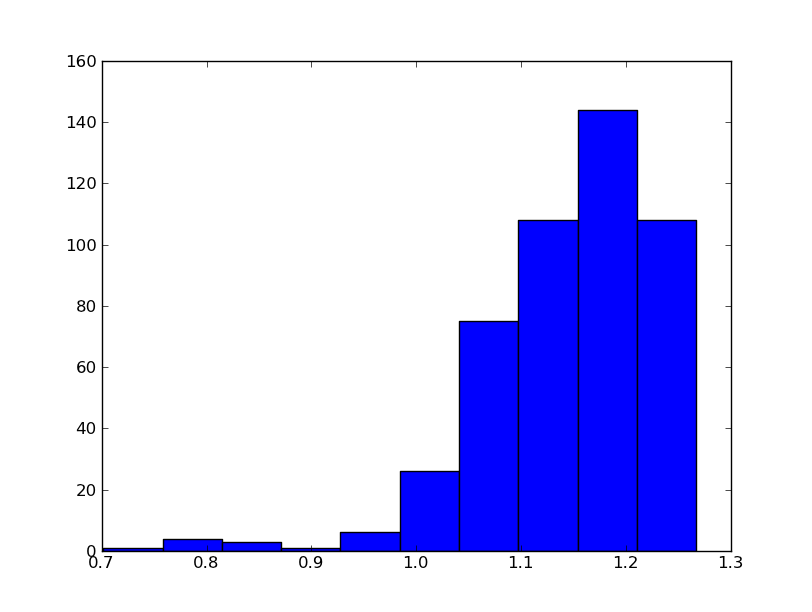
\includegraphics[width=0.9\linewidth]{mcmc500th1.png}
  \caption{Posterior distribution obtained for parameter $a$}
  \label{fig:t}
\end{subfigure}%
\begin{subfigure}{.54\linewidth}
  \centering
  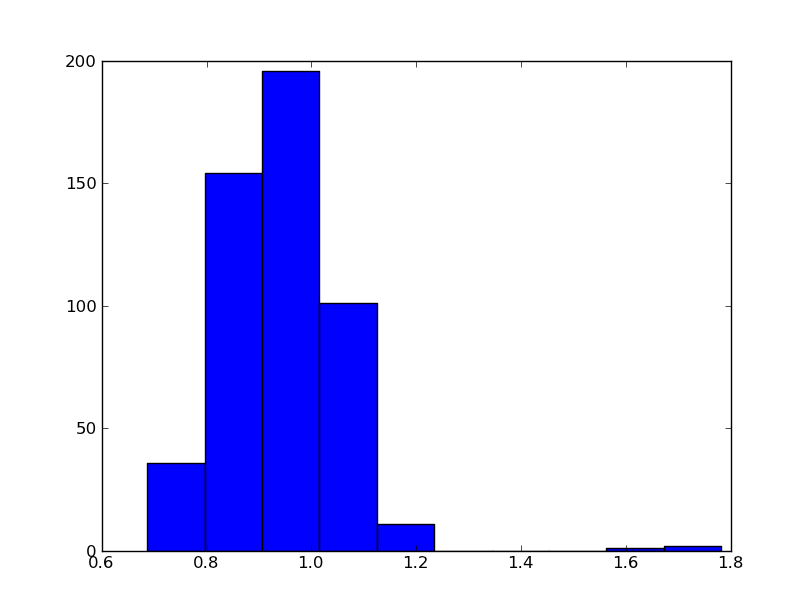
\includegraphics[width=0.9\linewidth]{mcmc500th2.png}
  \caption{Posterior distribution obtained for parameter $b$}
  \label{fig:ps}
\end{subfigure}
\caption{Posterior distribution inferred for parameters $a$ and $b$ with MCMC method(500 particles)}
\label{fig:mcmcdistros}
\end{figure}

Next, we applied the SMC algorithm with a manually tuned schedule $\epsilon = (30.0, 16.0, 6.0, \allowbreak5.0, 4.3)$. The prior distributions for model parameter $a$ and $b$ are taken to be uniform $a, b = \mathcal{U}(-10, 10)$. The perturbation kernels $K_{t}$ are taken to be Gaussian centered around the previous population and with standard deviation equal to that of the previous population. The results are shown in Figure~\ref{fig:smcres}. The evolution of the intermediate distributions for both parameters to the inferred distributions at $t=5$ is shown in Figure~\ref{smcinter}. It can be seen that the parameters are well inferred $a$: stats $b$: stats. The number of data generation steps needed for every intermediate population generated are shown in Table~\ref{dstep}. The numbers verify the claims in the previous section: the big difference between $\epsilon_{1}$ and $\epsilon_{2}$ is reflected in the big number of data generation steps needed to go from $t=1$ to $t=2$. On the other hand very few data generation steps are needed between $t=4$ and $t=5$ due to the small difference between $\epsilon_{4}$ and $\epsilon_{5}$.

\newpage
\begin{table}[ht]
\centering
\begin{tabular}{cc}
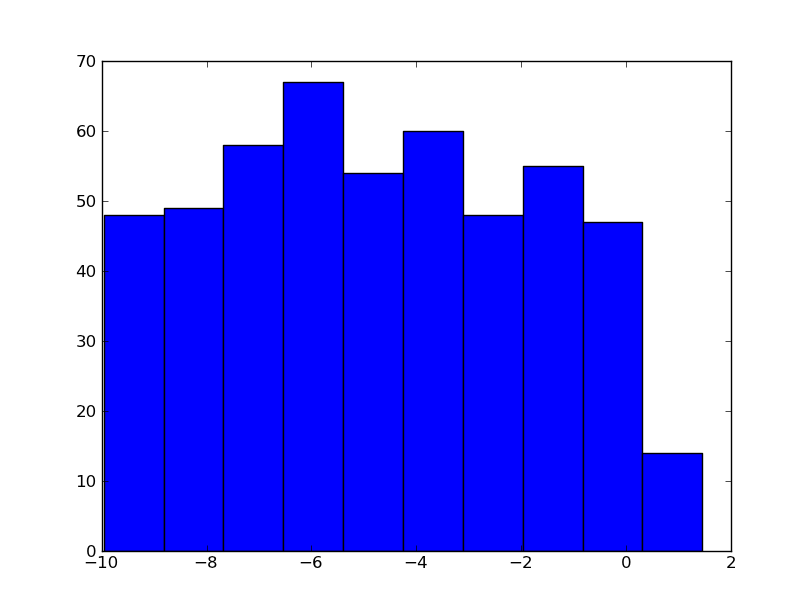
\includegraphics[scale=0.2]{p1th1_1}&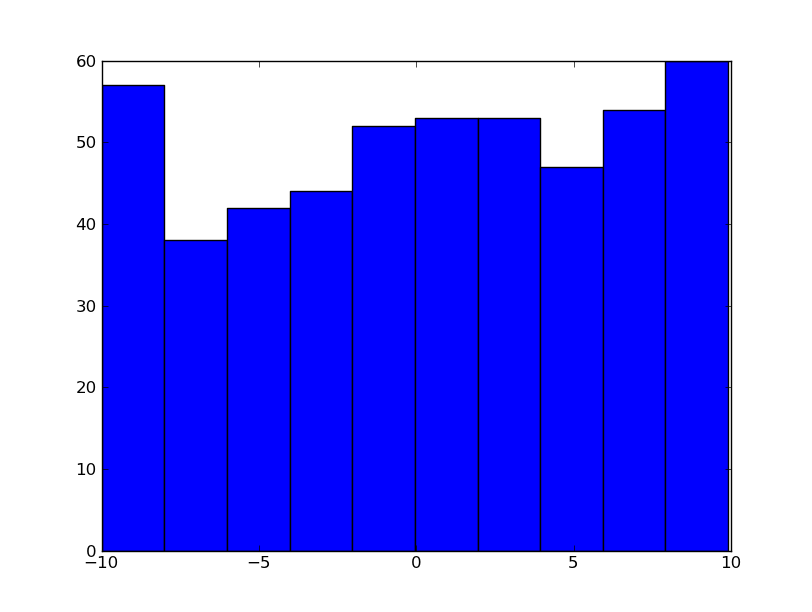
\includegraphics[scale=0.2]{p1th2_1.png}\\
\newline
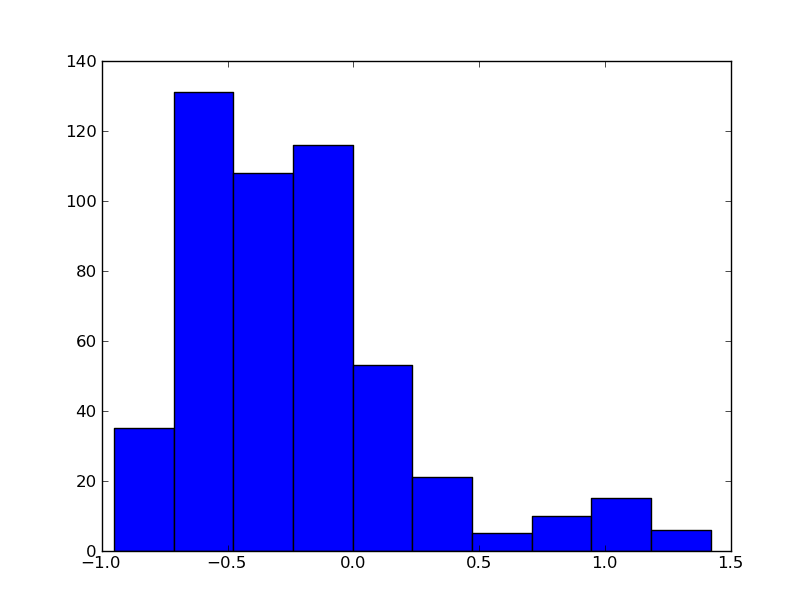
\includegraphics[scale=0.2]{p2th1_1}&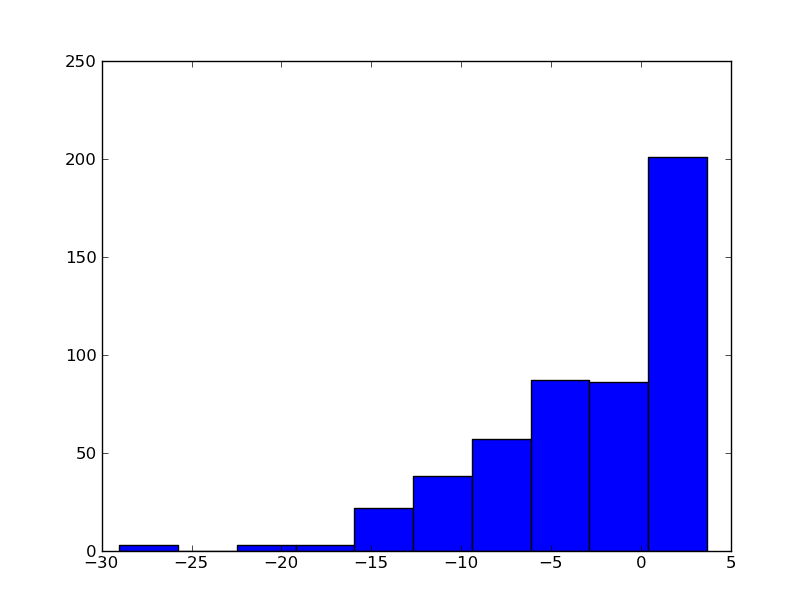
\includegraphics[scale=0.2]{p2th2_1.png}\\
\newline
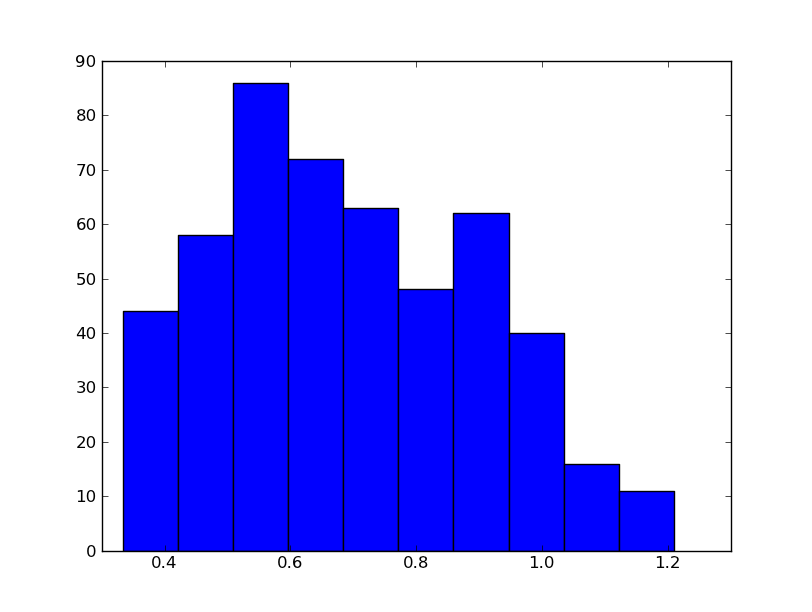
\includegraphics[scale=0.2]{p3th1_1}&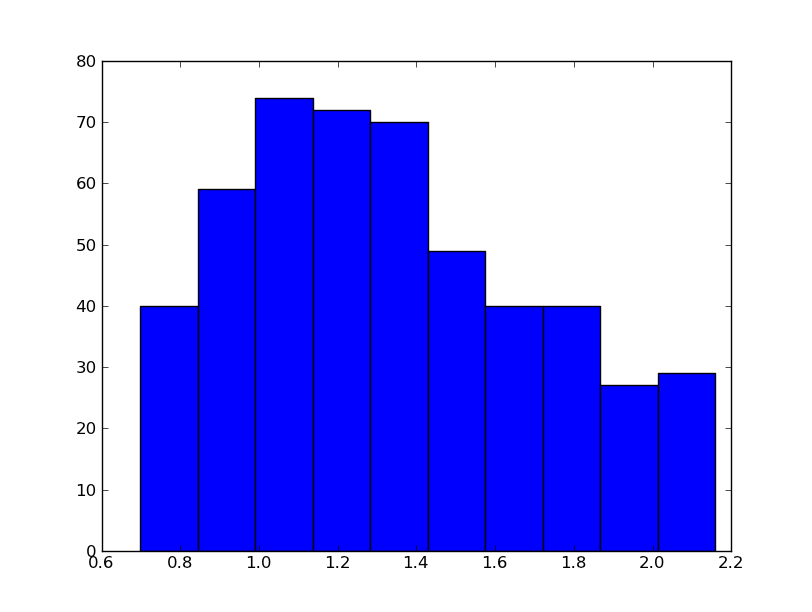
\includegraphics[scale=0.2]{p3th2_1.png}\\
\newline
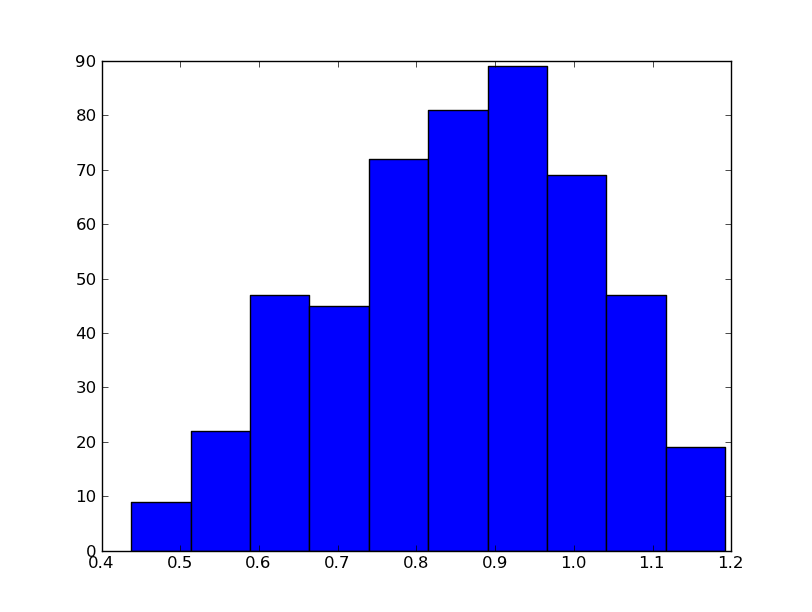
\includegraphics[scale=0.2]{p4th1_1}&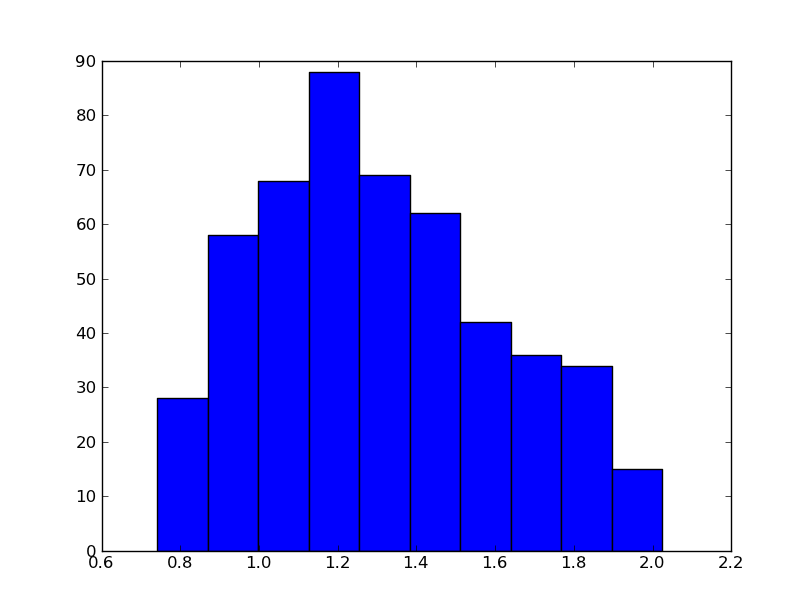
\includegraphics[scale=0.2]{p4th2_1.png}\\
\newline
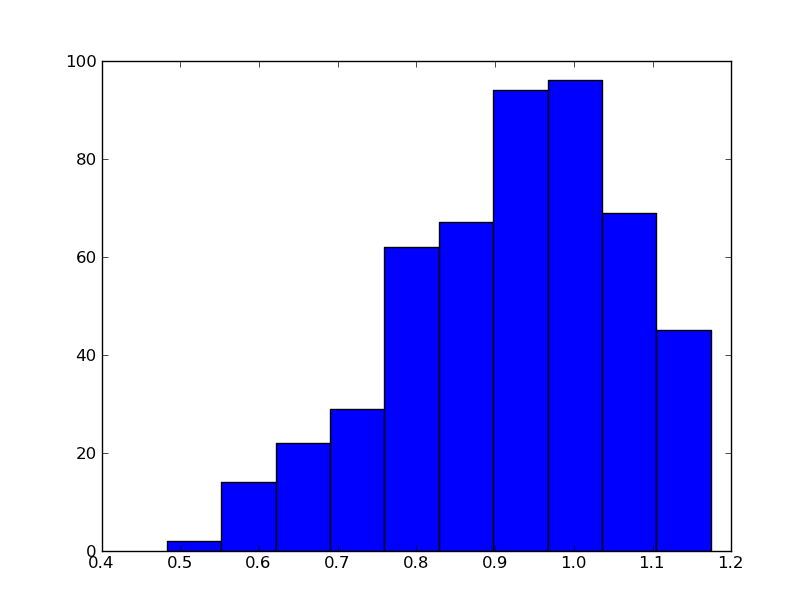
\includegraphics[scale=0.2]{p5th1_1}&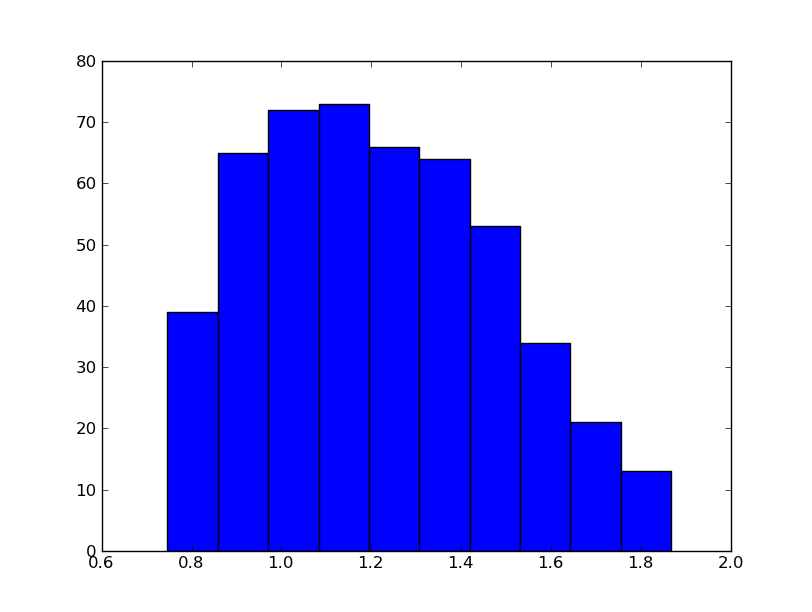
\includegraphics[scale=0.2]{p5th2_1.png}\\
\end{tabular}
\caption{Evolution of intermediate distribution for SMC method and $t=5$.}
\label{tab:smcinter}
\end{table}
\begin{table}[ht]
\centering
\begin{tabular}{ l*{5} c r }
\hline
population              & 1 & 2 & 3 & 4 & 5 \\
\hline
data generation steps & 926 & 13 563 & 50 135 & 51 214 & 52 411   \\
\hline
\end{tabular}
\caption{Cumulative data generation steps needed for each population.}
\label{tab:dsteps}
\end{table}
\begin{figure}
\centering
\begin{subfigure}{.52\linewidth}
  \centering
  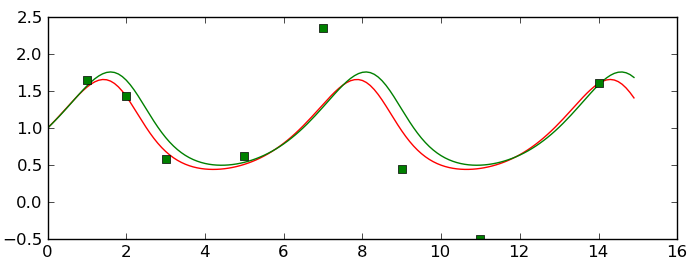
\includegraphics[scale=0.48]{smc500_x1.png}
  \caption{$x_{1}$}
  \label{fig:smcx1}
\end{subfigure}%
\begin{subfigure}{.5\linewidth}
  \centering
  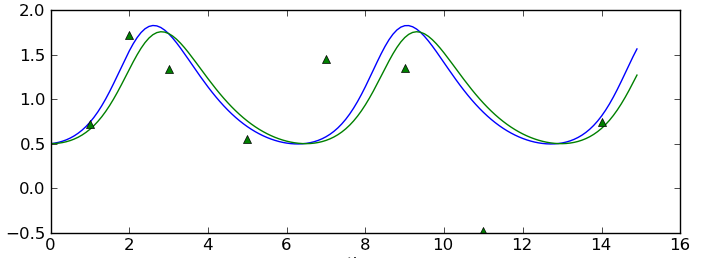
\includegraphics[scale=0.48]{smc500_x2.png}
  \caption{$x_{2}$}
  \label{fig:smcx2}
\end{subfigure}
\caption{Results for SMC method(500 particles). The green graphs are the ideal functions. The green triangles and squares are the noisy dataset used and the blue and red graphs are the inferred functions.}
\label{fig:smcres}
\end{figure}
\section{Future Work}
As stated in a previous section the main goals of the project were to create a tool that does automatic parameter estimation in dynamic biological systems and augment that by taking into account in the process other properties and characteristics of the systems such as evolution to make the inference process more powerful and the resulting models more complete. So far only the first part of task has been addressed, namely the automatic parameter estimation problem. The implemented algorithms could be refined by making better choices for the settings like using an adaptive $\epsilon$-schedule for the SMC algorithm and switch to Multivariate Gaussian distribution to account for correlations between parameters. 	The main bulk of the future work will however fall on the second task, incorporating the dynamic nature of these systems in the parameter inference process. One area of focus is accounting for evolutionary events like gene duplication. This could be a post-processing step which will act as model selection step after getting parameter candidates from the ABC procedures as described above. In order to get parameter candidates the algorithms will have to be tweaked because in their current state they give a population centered around a single value. One way to do it could be to employ some form of genetic algorithm of heuristic process to explore other areas of parameter space to get more parameters sets with high  likelihood. Then the model selection among models with the different candidate parameter sets will be done according to how well the competing models behave under evolutionary events such as gene duplication.
\bibliography{progress}
\appendix
\section{Time Management}
\begin{figure}[H]
\centering
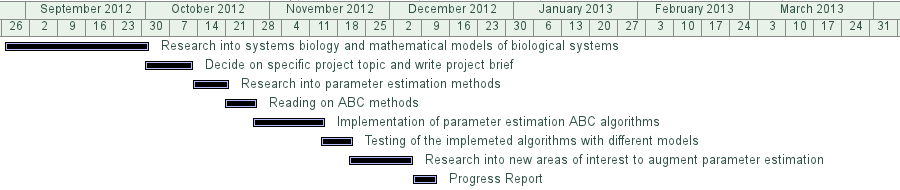
\includegraphics[scale=0.5]{gantt1}
\caption{Gantt chart for work so far}
\end{figure}
\begin{figure}[H]
\centering
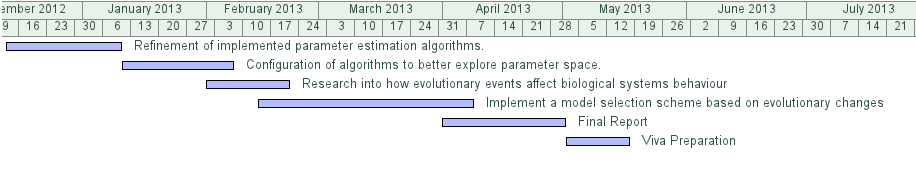
\includegraphics[scale=0.5]{gantt2}
\caption{Gantt chart for future work.}
\end{figure}
\end{document}